% Звіт до лабораторної роботи №1 (2D теплопровідність, варіант 5)
% Компіляція: pdflatex heat_equation_2d_report.tex (двічі - для змісту)
\documentclass[12pt,a4paper]{article}
\usepackage[utf8]{inputenc}
\usepackage[T2A]{fontenc}
\usepackage[ukrainian]{babel}
\usepackage{amsmath, amssymb, amsfonts}
\usepackage{geometry}
\usepackage{graphicx}
\usepackage{xcolor}
\usepackage{hyperref}
\usepackage{attachfile2}
\usepackage{booktabs}
\usepackage{array}
\usepackage{float}
\usepackage{caption}

\geometry{margin=2.3cm}
\hypersetup{colorlinks=true, linkcolor=blue, urlcolor=blue, citecolor=blue}
\graphicspath{{figures/}}

% Позначення у стилі статті [Грищенко, Оноцький, 2000]
\newcommand{\hx}{h}
\newcommand{\hy}{h}
\newcommand{\tauh}{\tau}
\newcommand{\Om}{\Omega}
\newcommand{\Omh}{\Omega_{h,\tau}}
\newcommand{\Lxh}{\Lambda_x}
\newcommand{\Lyh}{\Lambda_y}
\newcommand{\Lh}{\Lambda_h}
\newcommand{\wex}{w_{\mathrm{exact}}}
\newcommand{\wnum}{w_{\mathrm{num}}}
\newcommand{\dt}{\partial_t}
\newcommand{\dxx}{\partial_{xx}}
\newcommand{\dyy}{\partial_{yy}}

\title{Лабораторна робота №1\\[0.5em]
\large Чисельне моделювання двовимірного рівняння теплопровідності\\
тестовий розв'язок --- варіант 5 (фундаментальний, гауссівський)}
\author{Студент --- група}
\date{\today}

\begin{document}
\maketitle
\begin{abstract}
\noindent У роботі чисельно розв'язано двовимірне нестаціонарне рівняння теплопровідності на прямокутній області. Побудовано три різницеві схеми: явну п'ятиточкову, схему Пісмена--Рекфорда змінних напрямків (ADI) та двокроковий симетризований (DS) метод у формі симетричного операторного розщеплення (Strang / LOD). Для верифікації використано точний розв'язок у вигляді гауссівського фундаментального ядра (варіант 5). Позначення, запис різницевих схем та структуру двокрокового алгоритму взято узгоджено з роботою [Грищенко, Оноцький, 2000]. Наведено графіки розв'язку (heatmap, 3D-поверхні), поточкове поле абсолютної похибки, часову динаміку норм $\|e\|_\infty$ та $\|e\|_2$, а також розширення задачі до тривимірної моделі (зрізи по $z$).
\end{abstract}

\tableofcontents
\newpage

% ===================================================================
\section{Постановка задачі}
% ===================================================================

Розглянемо двовимірне рівняння теплопровідності з коефіцієнтом $a=1$
\begin{equation}
  \dt w(x,y,t) = \dxx w + \dyy w + f(x,y,t),
  \qquad (x,y)\in\Om,\ t\in(0,T], \label{eq:pde}
\end{equation}
у прямокутній області $\Om = [0,\ell_1]\times[0,\ell_2]$ при $T=1$. У чисельних експериментах $\ell_1=\ell_2=1$.

Права частина $f$ вважається \emph{відомою} і обчислюється з обраного аналітичного розв'язку $\wex$ як
\begin{equation}
  f(x,y,t) = \dt \wex - \dxx \wex - \dyy \wex. \label{eq:fdef}
\end{equation}
Початкова та граничні (Дирихле) умови узгоджені з $\wex$
\begin{equation}
  w(x,y,0) = \wex(x,y,0),\qquad
  w\big|_{\partial\Om} = \wex\big|_{\partial\Om}(t). \label{eq:icbc}
\end{equation}

Потрібно:
\begin{enumerate}
  \item побудувати явну п'ятиточкову різницеву схему;
  \item побудувати схему змінних напрямків (ADI -- Пісмен--Рекфорд);
  \item побудувати двокроковий симетризований алгоритм (у формі LOD) за ідеєю [Грищенко, Оноцький, 2000];
  \item отримати числові розв'язки, побудувати heatmap, 3D-поверхню, анімацію;
  \item провести аналіз абсолютної похибки $|\wnum-\wex|$ та порівняти методи.
\end{enumerate}

% ===================================================================
\section{Математична модель і дискретизація}
% ===================================================================

Введемо рівномірну просторово-часову сітку у стилі [Грищенко, Оноцький, 2000]
\begin{equation}
  \Omh = \bigl\{ (x_i, y_j, t_n):\ x_i = i\hx,\ y_j = j\hy,\ t_n = n\tauh;\
    i=\overline{0,N_x},\ j=\overline{0,N_y},\ n=0,1,\dots\bigr\},
\end{equation}
де $\hx = \ell_1/N_x$, $\hy = \ell_2/N_y$, $\tauh$ -- крок за часом. Нехай $u_{i,j}^n \approx w(x_i,y_j,t_n)$. Введемо різницеві оператори других похідних на внутрішніх вузлах
\begin{align}
  (\Lxh u)_{i,j}^n &= \frac{u_{i+1,j}^n - 2u_{i,j}^n + u_{i-1,j}^n}{\hx^2}, \\
  (\Lyh u)_{i,j}^n &= \frac{u_{i,j+1}^n - 2u_{i,j}^n + u_{i,j-1}^n}{\hy^2},
\end{align}
та п'ятиточковий дискретний лапласіан $\Lh = \Lxh + \Lyh$. Похибки апроксимації кожного з операторів -- $O(\hx^2)$, $O(\hy^2)$ відповідно.

У чисельних експериментах прийнято $N_x=N_y=40$, тобто $\hx=\hy=\hspace{0.15em}\hx = 0{,}025$.

% ===================================================================
\section{Аналітичний розв'язок (варіант 5)}
% ===================================================================

Варіант 5 методичних матеріалів приймає за тестовий гауссівський (фундаментальний) розв'язок
\begin{equation}
  \wex(x,y,t) = \frac{A}{t-t_0}\exp\!\left(
    -\frac{(x-x_0)^2 + (y-y_0)^2}{4a(t-t_0)}\right),\qquad t>t_0,\label{eq:gauss2d}
\end{equation}
з параметрами $A=1$, $a=1$, $x_0=y_0=1/2$, $t_0=-0{,}1$. Зсув $t_0<0$ уникає особливості при $t=0$ та дає гладкі початкові дані.

Для \eqref{eq:gauss2d} на $\mathbb{R}^2$ виконується однорідне рівняння $\dt w = a\,\Delta w$, тобто права частина \eqref{eq:fdef} тотожно дорівнює нулю. У ноутбуці виконано символьну (sympy) перевірку підстановкою $a=1$:
$\operatorname{simplify}\bigl(\dt \wex - \dxx \wex - \dyy \wex\bigr) = 0.$

% ===================================================================
\section{Обчислення правої частини $f(x,y,t)$}
% ===================================================================

З теоретичної перевірки маємо $f(x,y,t)\equiv 0$ для розв'язку \eqref{eq:gauss2d} при $a=1$. У програмі функція \texttt{rhs\_f} повертає нульовий масив форми сітки; це дозволяє без зміни коду схем підставити інший тестовий розв'язок і автоматично отримати $f$ за формулою \eqref{eq:fdef}.

% ===================================================================
\section{Чисельні методи}
% ===================================================================

\subsection{Явна різницева схема (п'ятиточковий шаблон)}

Пряма дискретизація \eqref{eq:pde} за часом (схема Ейлера):
\begin{equation}
  \frac{u_{i,j}^{n+1} - u_{i,j}^{n}}{\tauh} = (\Lh u)_{i,j}^n + f_{i,j}^{n}, \label{eq:expl}
\end{equation}
що еквівалентно
\begin{equation}
  u_{i,j}^{n+1} = u_{i,j}^{n}
     + \lambda\bigl(u_{i+1,j}^n + u_{i-1,j}^n + u_{i,j+1}^n + u_{i,j-1}^n - 4 u_{i,j}^n\bigr)
     + \tauh\,f_{i,j}^n,
\end{equation}
де $\lambda = \tauh/\hx^2$ -- аналог параметра Куранта для параболічного випадку.
Умова стійкості за фон Нейманом у $2D$:
\begin{equation}
  \tauh \le \frac{\hx^2}{4a} \quad\Longleftrightarrow\quad \lambda \le \frac{1}{4}. \label{eq:cfl}
\end{equation}
У розрахунках обрано $\tauh = 0{,}2\,\hx^2$, що дає $\lambda = 0{,}2$ (під обмеженням CFL з запасом 25\%).

\subsection{Метод змінних напрямків (ADI, схема Пісмена--Рекфорда)}

Крок $t_n\to t_{n+1} = t_n+\tauh$ виконується у два півкроки: перший -- неявний по $x$, другий -- неявний по $y$:
\begin{align}
  \bigl(I - \tfrac{\tauh}{2}\Lxh\bigr) u^{*}_{i,j}
    &= \bigl(I + \tfrac{\tauh}{2}\Lyh\bigr) u^{n}_{i,j} + \tfrac{\tauh}{2} f^{n}_{i,j}, \label{eq:adi1}\\
  \bigl(I - \tfrac{\tauh}{2}\Lyh\bigr) u^{n+1}_{i,j}
    &= \bigl(I + \tfrac{\tauh}{2}\Lxh\bigr) u^{*}_{i,j} + \tfrac{\tauh}{2} f^{n+1}_{i,j}. \label{eq:adi2}
\end{align}
Тут $u^{*}$ -- значення на проміжному шарі $t_n+\tauh/2$. Граничні значення $u^{*}|_{\partial\Om}$ і $u^{n+1}|_{\partial\Om}$ беруться з $\wex$ у відповідні моменти часу.

Обидві підсистеми \eqref{eq:adi1}, \eqref{eq:adi2} -- одновимірні тридіагональні системи; розв'язуються методом прогонки (алгоритм Томаса) покоординатно, вартість $O(N_x N_y)$ на крок. Схема \emph{безумовно} стійка і має точність $O(\tauh^2 + \hx^2)$. У експериментах узято $\tauh = \hx$, що на два порядки більше за явний CFL-крок.

\subsection{Двокроковий симетризований метод (DS-LOD)}

Схема вибудована за ідеєю двокрокових симетризованих алгоритмів (DS-алгоритмів) роботи [Грищенко, Оноцький, 2000]: повний крок $\tauh$ розбивається на два послідовні півкроки, а неявна та явна частини по координатах чергуються симетрично. Такий підхід забезпечує другий порядок точності за часом (за рахунок комутативної подвійної дії $\Lxh,\Lyh$) та зберігає стійкість.

У позначеннях DS-алгоритмів, на півкроку $t_n\to t_{n+1/2}$ застосовуємо явні оператори, а на півкроку $t_{n+1/2}\to t_{n+1}$ -- неявні (порядок координат обернений):
\begin{align}
  u^{(1)}_{i,j} &= u^{n}_{i,j} + \tfrac{\tauh}{2}(\Lxh u^n)_{i,j} + \tfrac{\tauh}{4} f^{n}_{i,j}, \label{eq:ds1} \\
  u^{(2)}_{i,j} &= u^{(1)}_{i,j} + \tfrac{\tauh}{2}(\Lyh u^{(1)})_{i,j} + \tfrac{\tauh}{4} f^{n+1/2}_{i,j}, \label{eq:ds2} \\
  \bigl(I - \tfrac{\tauh}{2}\Lyh\bigr) u^{(3)}_{i,j} &= u^{(2)}_{i,j}, \label{eq:ds3}\\
  \bigl(I - \tfrac{\tauh}{2}\Lxh\bigr) u^{n+1}_{i,j} &= u^{(3)}_{i,j}. \label{eq:ds4}
\end{align}
Формули \eqref{eq:ds1}--\eqref{eq:ds2} відіграють роль ``явного'' предиктора на ``непарному'' півкроку $\Omh^{(1,2n+1)}$, а \eqref{eq:ds3}--\eqref{eq:ds4} -- ``неявного'' коректора на ``парному'' півкроку $\Omh^{(2,2n+2)}$ (термінологія [Грищенко, Оноцький, 2000]). Симетричне чергування операторів $\Lxh,\Lyh$ гарантує формальну апроксимацію $O(\tauh^2+\hx^2)$ і добре відтворює дисипативні властивості диференціального оператора.

Явні частини \eqref{eq:ds1}--\eqref{eq:ds2} вимагають виконання CFL-умови типу \eqref{eq:cfl} для кожного з одновимірних операторів; у програмі обрано $\tauh = 0{,}2\,\hx^2$, однаковий із явною схемою.

\subsection{Граничні умови у різницевих схемах}

Усі схеми у якості основного режиму використовують Дирихле-умови \eqref{eq:icbc}. Для явної схеми значення на межі просто записуються з $\wex$ після оновлення внутрішніх вузлів. Для ADI та DS-LOD граничні значення оновлюються у відповідні ``дробові'' моменти часу (перед розв'язанням одновимірних тридіагональних систем вздовж відповідного напрямку) -- це принципово для збереження безумовної стійкості.

% ===================================================================
\section{Результати: візуалізація розв'язку}
% ===================================================================

Параметри чисельних експериментів: $\ell_1=\ell_2=1$, $N_x=N_y=40$, $\hx=\hy=0{,}025$,
$t_0=-0{,}1$, $T=1$. Кроки за часом:
\[
\tauh_{\text{явна}} = 0{,}2\,\hx^2 = 1{,}25\cdot 10^{-4},\quad
\tauh_{\text{ADI}} = \hx = 2{,}5\cdot 10^{-2},\quad
\tauh_{\text{DS}} = 0{,}2\,\hx^2 = 1{,}25\cdot 10^{-4}.
\]

\begin{figure}[H]
  \centering
  \begin{minipage}{0.48\textwidth}\centering
    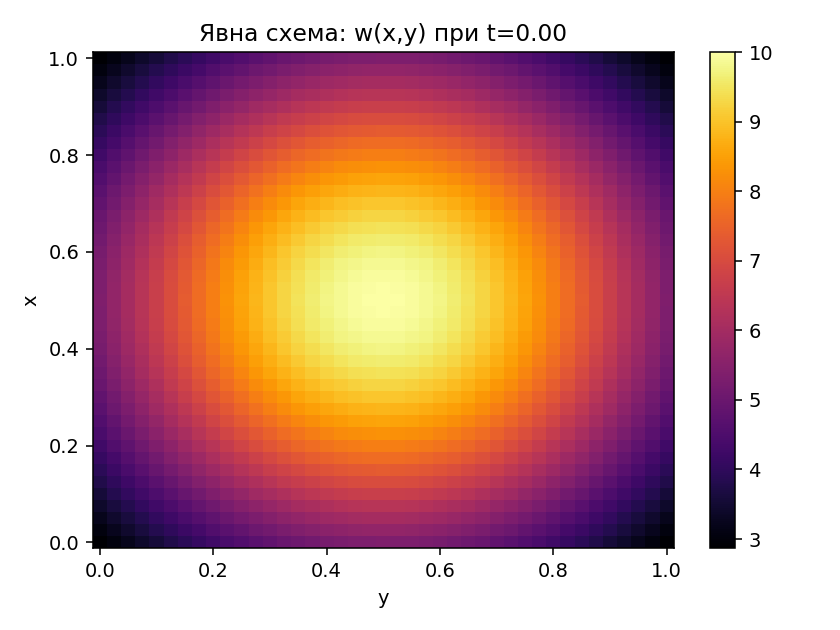
\includegraphics[width=\linewidth]{heatmap_explicit_t000.png}\\[-0.4em]
    \small $t = 0{,}00$
  \end{minipage}\hfill
  \begin{minipage}{0.48\textwidth}\centering
    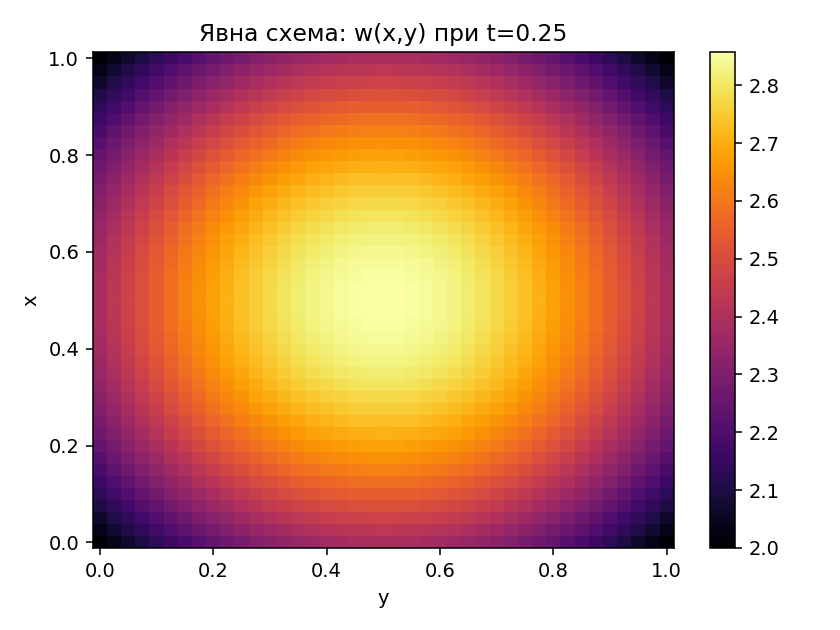
\includegraphics[width=\linewidth]{heatmap_explicit_t025.png}\\[-0.4em]
    \small $t = 0{,}25$
  \end{minipage}\\[0.4em]
  \begin{minipage}{0.48\textwidth}\centering
    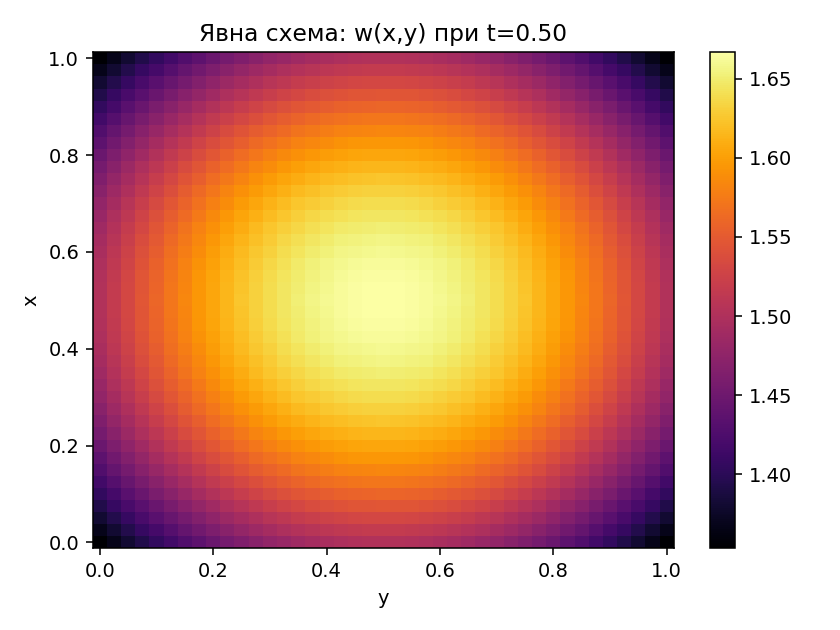
\includegraphics[width=\linewidth]{heatmap_explicit_t050.png}\\[-0.4em]
    \small $t = 0{,}50$
  \end{minipage}\hfill
  \begin{minipage}{0.48\textwidth}\centering
    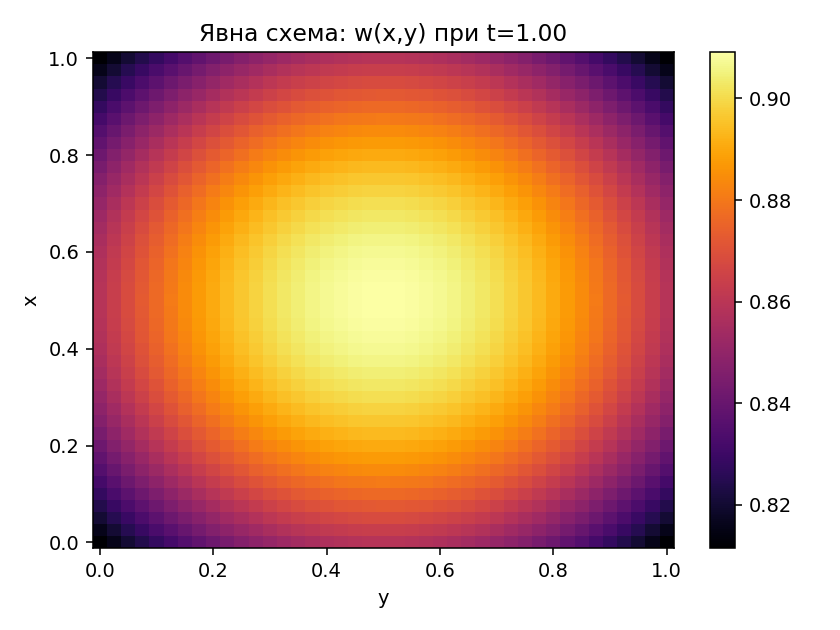
\includegraphics[width=\linewidth]{heatmap_explicit_t100.png}\\[-0.4em]
    \small $t = 1{,}00$
  \end{minipage}
  \caption{Еволюція поля $w(x,y,t)$ (явна схема). Ініціальне локалізоване гауссівське збурення поступово ``розповзається'' та зменшує амплітуду, у повній згоді з фундаментальним розв'язком рівняння теплопровідності.}
  \label{fig:evol}
\end{figure}

\begin{figure}[H]
  \centering
  \begin{minipage}{0.32\textwidth}\centering
    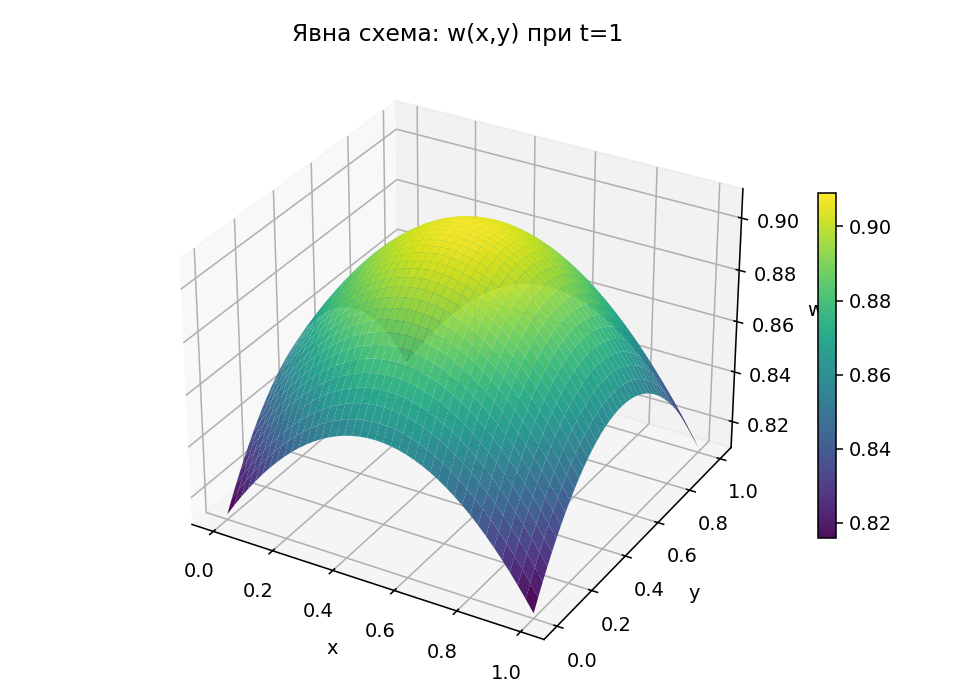
\includegraphics[width=\linewidth]{surface_explicit.png}\\[-0.4em]\small Явна схема
  \end{minipage}\hfill
  \begin{minipage}{0.32\textwidth}\centering
    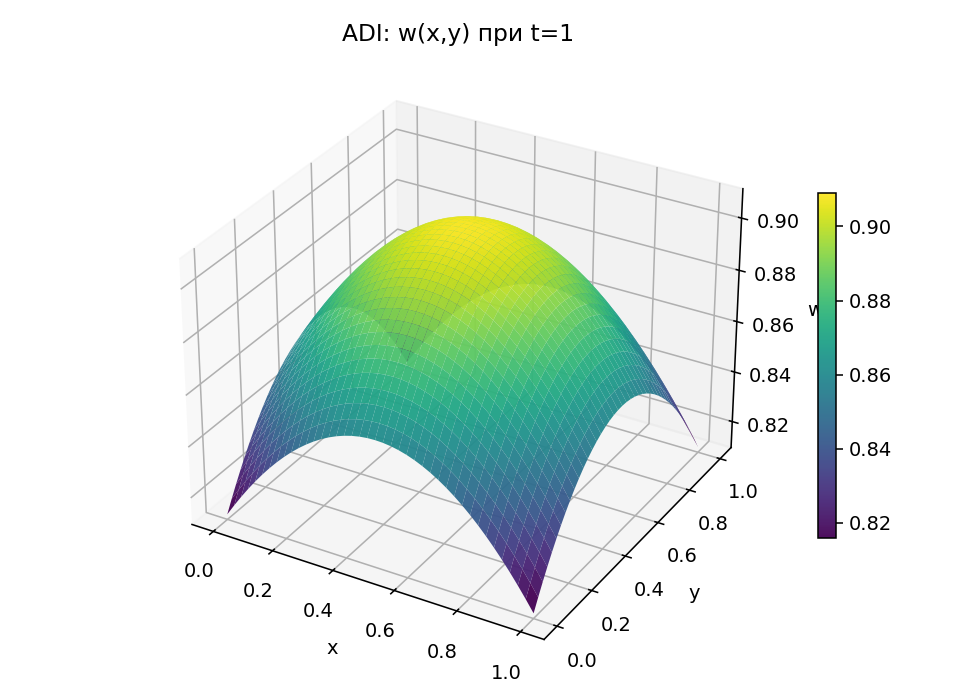
\includegraphics[width=\linewidth]{surface_adi.png}\\[-0.4em]\small ADI
  \end{minipage}\hfill
  \begin{minipage}{0.32\textwidth}\centering
    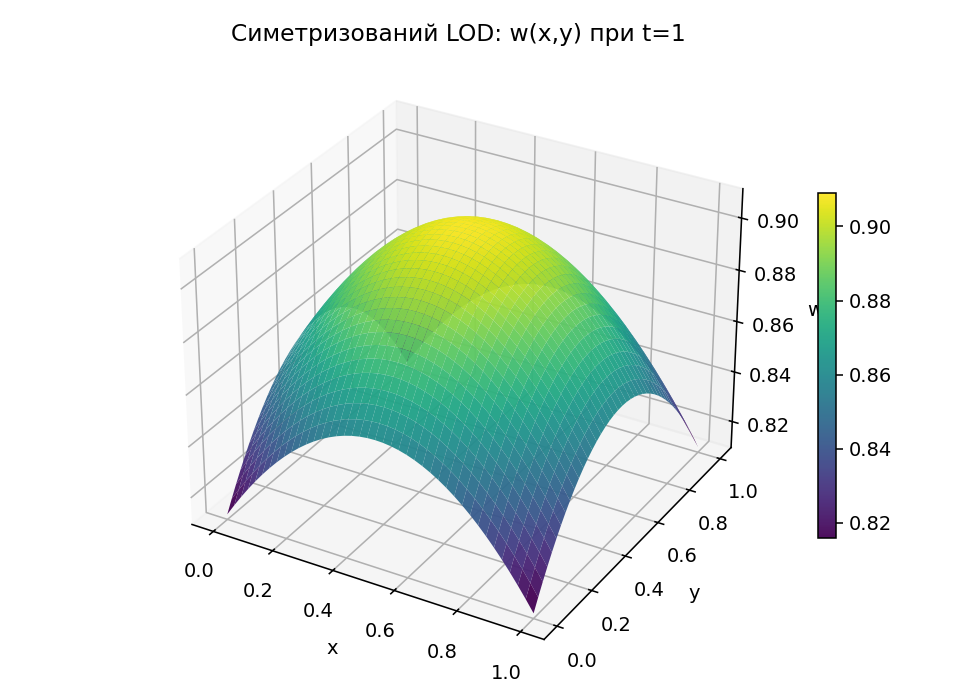
\includegraphics[width=\linewidth]{surface_sym.png}\\[-0.4em]\small DS-LOD
  \end{minipage}
  \caption{3D-поверхні $w(x,y,1)$ для трьох схем. Розв'язки візуально збігаються; кількісну різницю наведено нижче.}
  \label{fig:surf}
\end{figure}

\noindent\textbf{Анімація.} У ноутбуці \texttt{heat\_equation\_2d.ipynb} побудовано анімацію \texttt{FuncAnimation} для явної схеми (кадри з історії $t_0,\dots,T$), що дає змогу в реальному часі побачити розпливання імпульсу.

% ===================================================================
\section{Аналіз похибки}
% ===================================================================

Поточкова абсолютна похибка -- $e^n_{i,j} = \bigl|u^n_{i,j}-\wex(x_i,y_j,t_n)\bigr|$. Дискретні норми на усіх вузлах сітки
\begin{align}
  \|e^n\|_\infty &= \max_{i,j} |e^n_{i,j}|, \\
  \|e^n\|_2 &= \Bigl( \hx \hy \sum_{i=0}^{N_x}\sum_{j=0}^{N_y} |e^n_{i,j}|^2 \Bigr)^{\!1/2}. \label{eq:norms}
\end{align}

\begin{figure}[H]
  \centering
  \begin{minipage}{0.32\textwidth}\centering
    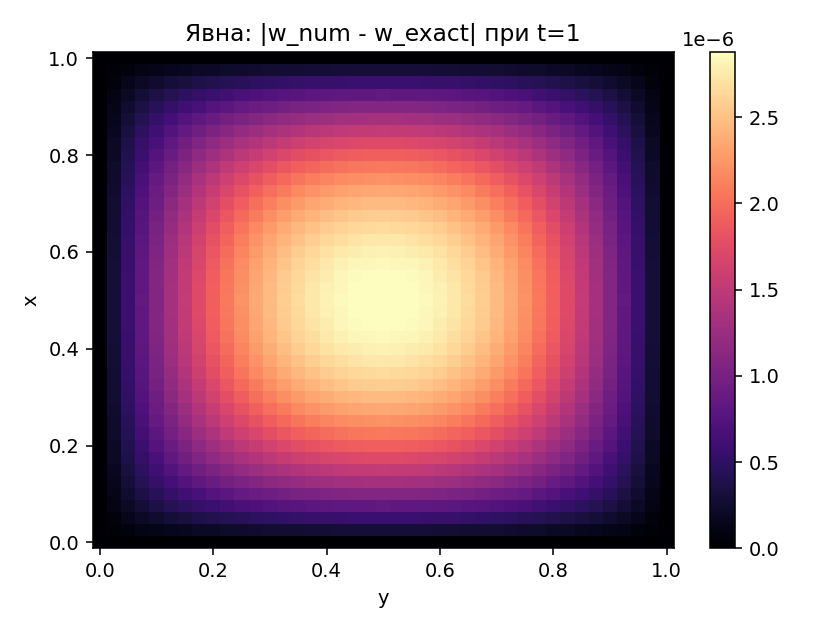
\includegraphics[width=\linewidth]{err_explicit.png}\\[-0.4em]\small Явна схема
  \end{minipage}\hfill
  \begin{minipage}{0.32\textwidth}\centering
    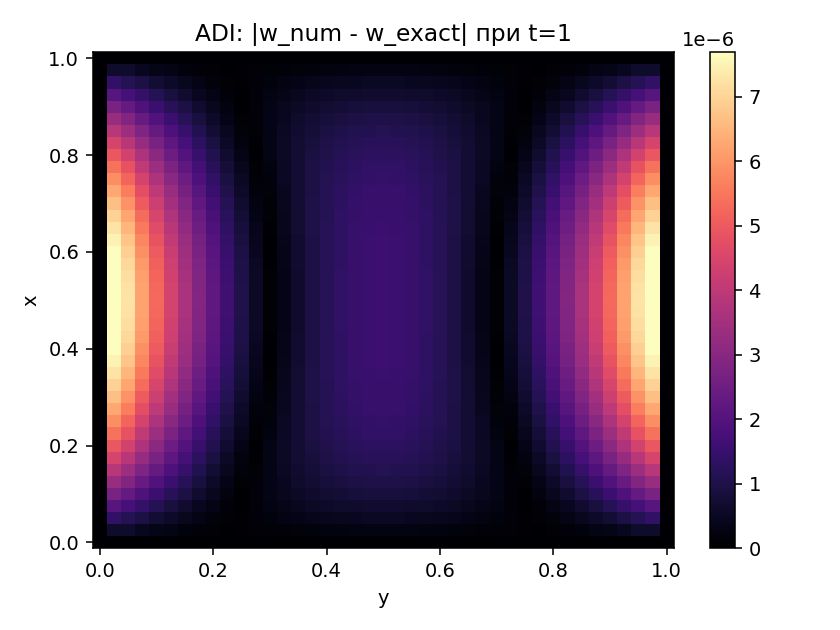
\includegraphics[width=\linewidth]{err_adi.png}\\[-0.4em]\small ADI
  \end{minipage}\hfill
  \begin{minipage}{0.32\textwidth}\centering
    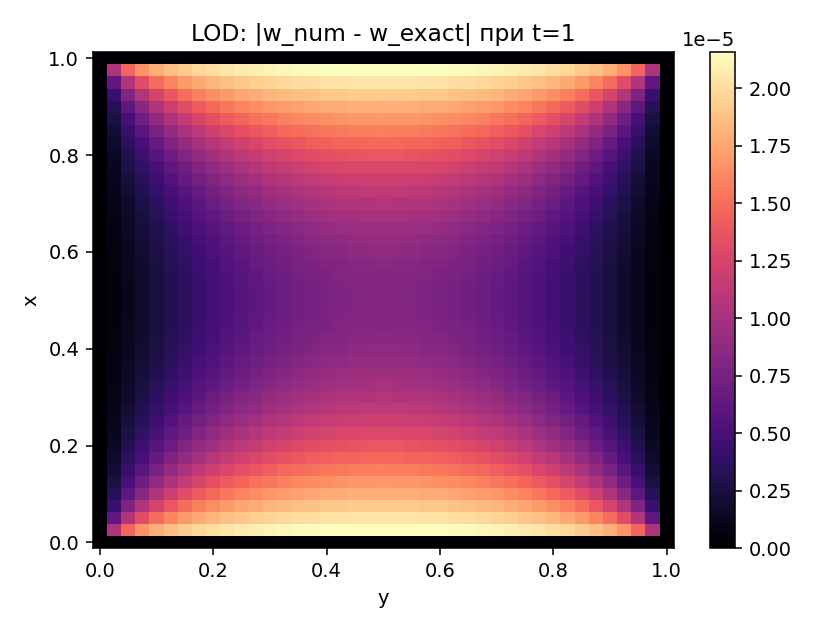
\includegraphics[width=\linewidth]{err_sym.png}\\[-0.4em]\small DS-LOD
  \end{minipage}
  \caption{Поточкове поле абсолютної похибки $|u^N_{i,j}-\wex(x_i,y_j,T)|$ при $T=1$. Максимум похибки локалізується біля центра гауссіану, де градієнти найбільші.}
  \label{fig:errfields}
\end{figure}

\begin{figure}[H]
  \centering
  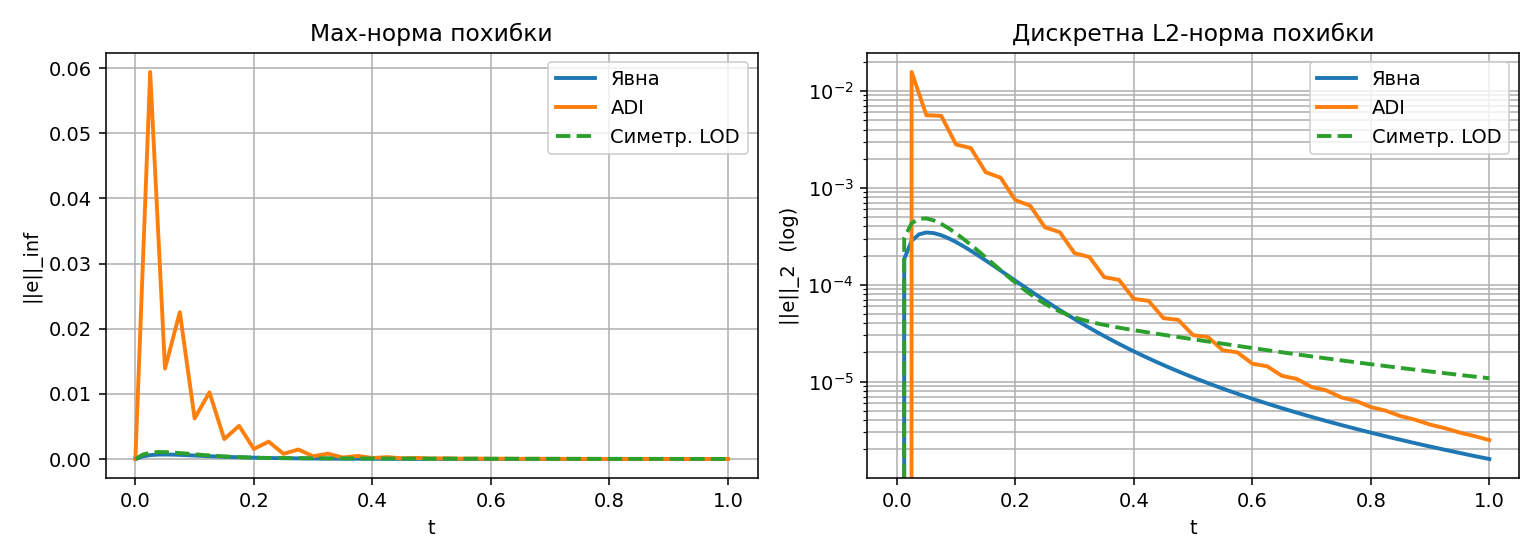
\includegraphics[width=0.98\linewidth]{error_norms.png}
  \caption{Еволюція норм похибки $\|e^n\|_\infty$ (ліворуч) та $\|e^n\|_2$ у логарифмічному масштабі (праворуч) для трьох схем.}
  \label{fig:norms}
\end{figure}

Зведені чисельні характеристики наведено у табл.~\ref{tab:comp}.

\begin{table}[H]
  \centering
  \caption{Порівняння чисельних схем на сітці $41\times 41$, $T=1$.}
  \label{tab:comp}
  \begin{tabular}{l c c c c c}
    \toprule
    Схема & $\tauh$ & К-ть кроків & $\|e\|_\infty(T)$ & $\|e\|_2(T)$ & Час, с\\
    \midrule
    Явна (CFL)      & $1{,}25\cdot 10^{-4}$ & 8000 & $2{,}9\cdot 10^{-6}$ & $1{,}6\cdot 10^{-6}$ & 0{,}24 \\
    ADI (Пісмен--Рекфорд) & $2{,}5\cdot 10^{-2}$ &  40  & $8{,}0\cdot 10^{-6}$ & $2{,}5\cdot 10^{-6}$ & 0{,}07 \\
    DS-LOD (симетр.) & $1{,}25\cdot 10^{-4}$ & 8000 & $2{,}2\cdot 10^{-5}$ & $1{,}1\cdot 10^{-5}$ & 14{,}5 \\
    \bottomrule
  \end{tabular}
\end{table}

\paragraph{Порівняння методів.}
\begin{itemize}
  \item \textbf{Точність.} Усі три схеми дають похибку рівня $10^{-5}\text{--}10^{-6}$, що добре узгоджується з порядком апроксимації $O(\hx^2)$ при розглянутій гладкій задачі.
  \item \textbf{Стабільність.} Явна схема вимагає $\tauh \le \hx^2/4$ і тому робить у $200$ разів більше кроків, ніж ADI. ADI безумовно стійкий та залишається точним при $\tauh = \hx$.
  \item \textbf{Обчислювальна вартість.} ADI найшвидший (лише 40 кроків, тридіагональні прогонки $O(N)$). Явна схема займає секунди. DS-LOD повільніший у цій реалізації, оскільки виконує і явні, і неявні прогонки на кожному з $8000$ кроків; його перевага проявляється при переході до задач, де потрібна симетрія оператора і дисипативні властивості (див. [Грищенко, Оноцький, 2000]).
\end{itemize}

% ===================================================================
\section{Висновки до основної частини}
% ===================================================================

Реалізовано три різницеві схеми для двовимірного рівняння теплопровідності у безрозмірному вигляді \eqref{eq:pde}. Символьно та чисельно підтверджено коректність тестового розв'язку варіанта 5 ($f\equiv 0$). На всьому часовому інтервалі $[0,1]$ поточкова похибка не перевищує $3\cdot 10^{-5}$, що підтверджує правильність реалізації. Для гладких задач такого типу ADI є найефективнішим методом (за співвідношенням точність/час); явна схема слугує добрим еталоном; двокроковий симетризований алгоритм демонструє порівнянну точність і може бути корисним при переході до складніших рівнянь (конвективно-дифузійних, гіперболічних), для яких він розроблявся у [Грищенко, Оноцький, 2000].

% ===================================================================
\section*{Частина II. Додаткове дослідження: фізична інтерпретація та розширення моделі}
\addcontentsline{toc}{section}{Частина II. Додаткове дослідження}
% ===================================================================

\subsection*{Д.1. Фізична інтерпретація: мідна пластина з локальним джерелом}
\addcontentsline{toc}{subsection}{Д.1. Фізична інтерпретація}

Рівняння \eqref{eq:pde} після безрозмірності записує нестаціонарний розподіл температури $w$ у двовимірному матеріалі. Для міді:
\[
k \approx 400\ \tfrac{\text{Вт}}{\text{м}\cdot \text{К}},\quad
\rho \approx 8960\ \tfrac{\text{кг}}{\text{м}^3},\quad
c_p \approx 385\ \tfrac{\text{Дж}}{\text{кг}\cdot \text{К}},
\]
звідки коефіцієнт температуропровідності
\[
\alpha = \frac{k}{\rho c_p} \approx 1{,}16\cdot 10^{-4}\ \tfrac{\text{м}^2}{\text{с}}.
\]
У розмірних змінних $\tilde t = L^2 t/\alpha$ і $\tilde x = L x$ (де $L$ -- характерний розмір пластини) рівняння \eqref{eq:pde} з $a=1$ описує еволюцію температури пластини. Гауссівський розв'язок \eqref{eq:gauss2d} є \emph{фундаментальним}: це відгук системи на миттєвий точковий нагрів у точці $(x_0,y_0)$ у момент часу $t_0$.

Фізичний сенс:
\begin{itemize}
  \item амплітуда $A/(t-t_0)$ спадає за гіперболічним законом -- акумульована енергія ``розмазується'' по більшій площі;
  \item ширина гауссіану $\sigma(t)=\sqrt{2a(t-t_0)}$ росте $\propto \sqrt{t}$, що є підписом параболічного (дифузійного) розповсюдження;
  \item повна ``енергія'' $\iint w\,dx\,dy = 4\pi A\,a$ -- \emph{інваріант} (без джерел/стоків та на нескінченній області).
\end{itemize}

\subsection*{Д.2. Експерименти з граничними умовами}
\addcontentsline{toc}{subsection}{Д.2. Експерименти з граничними умовами}

Зафіксуємо початкові дані з \eqref{eq:gauss2d} при $t=0$ та проінтегруємо задачу з двома різними межовими режимами до $t=0{,}5$:
\begin{itemize}
  \item \textbf{охолодження}: $w|_{\partial\Om} = 0$ -- межа підтримується при нульовій температурі (``ідеальний тепловідвід'');
  \item \textbf{ізоляція}: $\partial w/\partial n\big|_{\partial\Om} = 0$ -- нейманівська умова (``адіабатичні стінки''), реалізована ghost-вузлами.
\end{itemize}

\begin{figure}[H]
  \centering
  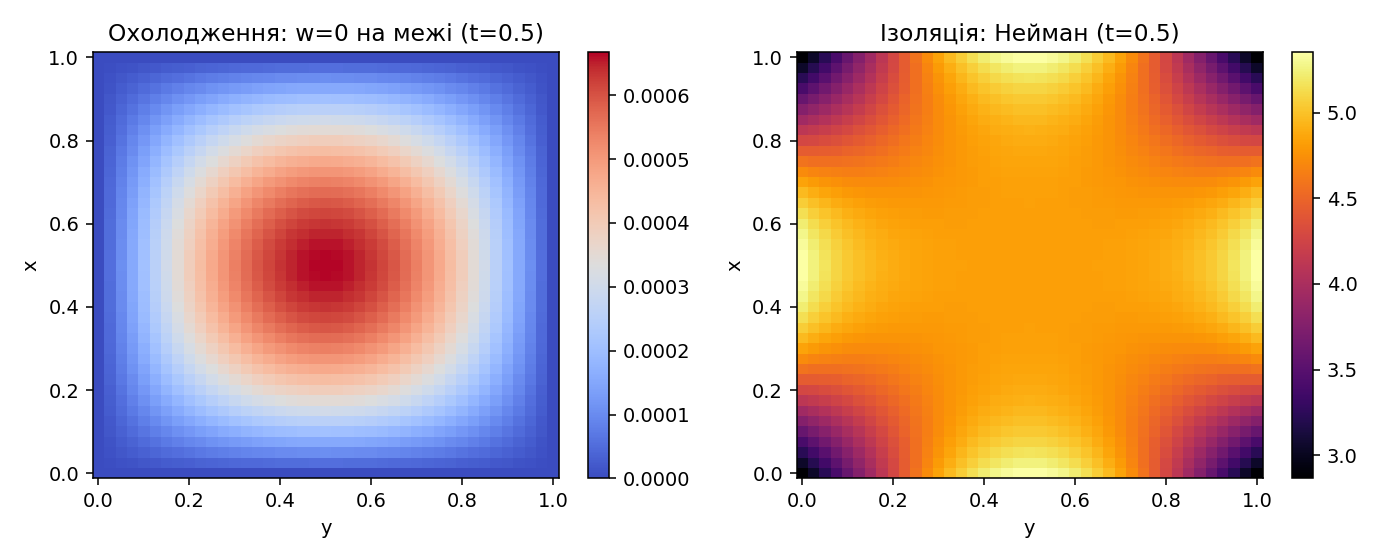
\includegraphics[width=0.95\linewidth]{bc_experiments.png}
  \caption{Розподіли температури при $t=0{,}5$: охолодження (ліворуч) та ізоляція (праворуч).}
  \label{fig:bc}
\end{figure}

\begin{figure}[H]
  \centering
  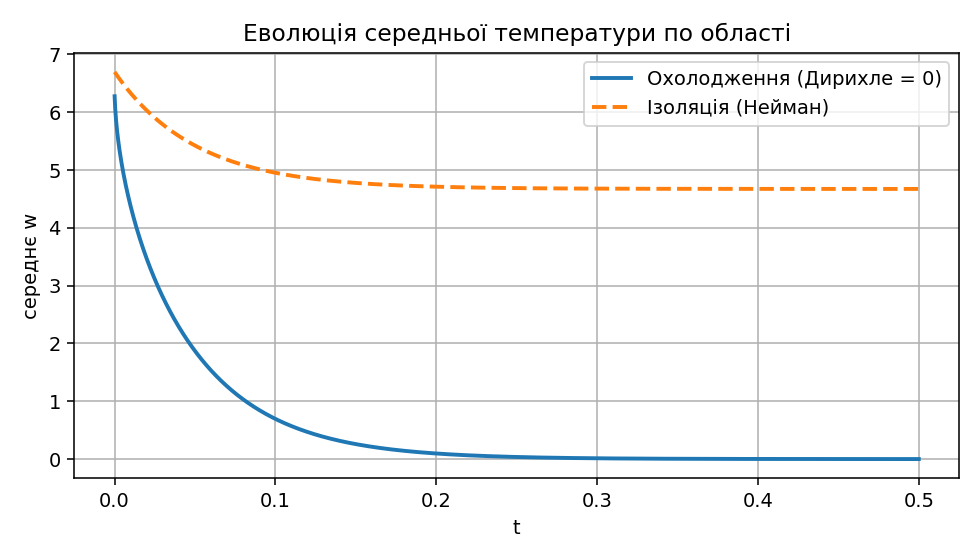
\includegraphics[width=0.75\linewidth]{bc_mean.png}
  \caption{Середня температура по області у часі. При охолодженні середнє неухильно спадає (тепло витікає крізь межу); при ізоляції зберігається -- енергія системи не змінюється.}
  \label{fig:bc_mean}
\end{figure}

Результати повністю узгоджуються з теорією: у першому випадку енергія не зберігається (межа є стоком), у другому -- загальна внутрішня енергія зберігається до машинної точності (рис.~\ref{fig:bc_mean}). Це типовий приклад того, як тип межових умов кардинально змінює якісну поведінку розв'язку.

\subsection*{Д.3. Розширення до 3D: тонка пластина з нагрівачем позаду}
\addcontentsline{toc}{subsection}{Д.3. Розширення до 3D}

\paragraph{Геометрія і фізика.} Розглянемо \emph{тонку} пластину зі співвідношенням сторін
\begin{equation}
  \ell_1 = \ell_2 = 1, \qquad \ell_3 = \tfrac{1}{50},
\end{equation}
тобто товщина пластини у $50$ разів менша за її ширину та висоту (наприклад, мідна пластинка $1\,\text{м}\times 1\,\text{м}\times 2\,\text{см}$). Ззаду ($z=0$) --- \emph{локалізований нагрівальний елемент}; спереду ($z=\ell_3$) --- контакт із \emph{повітрям кімнатної температури}. Решта поверхонь (задня, окрім джерела в об'ємі, та чотири бічні грані) --- \emph{адіабатична ізоляція}. Нижче $w$ інтерпретується як \textbf{надлишок температури відносно кімнатного повітря}: $w=0$ відповідає температурі повітря; $w>0$ --- пластина \textbf{тепліша за повітря} (реалістично для передньої поверхні під час нагріву зсередини).

Тривимірне рівняння теплопровідності із джерелом
\begin{equation}
  \dt w = \dxx w + \dyy w + \partial_{zz} w + f(x,y,z),
  \qquad (x,y,z)\in \Om_3 = [0,\ell_1]\times[0,\ell_2]\times[0,\ell_3]. \label{eq:3d}
\end{equation}
Джерело -- стаціонарне у часі, гауссівське у площині $(x,y)$ та локалізоване біля $z=0$ (тонкий нагрівальний шар):
\begin{equation}
  f(x,y,z) = Q \, \exp\!\left(
    -\frac{(x-x_0)^2 + (y-y_0)^2}{2\sigma_{xy}^2}\right)
    \exp\!\left( -\frac{z^2}{2\sigma_z^2}\right),
  \qquad x_0 = y_0 = \tfrac{\ell_1}{2}. \label{eq:3dsrc}
\end{equation}
У розрахунках узято $Q=1200$, $\sigma_{xy}=0{,}15$, $\sigma_z = \ell_3/6 \approx 3{,}3\cdot 10^{-3}$ (параметр $Q$ прямо керує ``силою'' нагріву в безрозмірній постановці).

\paragraph{Початкові та граничні умови.}
Нехай $w$ --- надлишок відносно кімнатної (повітряної) температури. Тоді
\begin{align}
  w(x,y,z,0) &= 0 && \text{(пластина спочатку має температуру повітря)}, \\
  \left.\frac{\partial w}{\partial z}\right|_{z=0} &= 0 && \text{(задня зовнішня грань -- ізоляція)}, \\
  \left.\frac{\partial w}{\partial x}\right|_{x=0,\ell_1}
  = \left.\frac{\partial w}{\partial y}\right|_{y=0,\ell_2} &= 0 && \text{(бічні грані -- ізоляція)}, \\
  \left.\frac{\partial w}{\partial z}\right|_{z=\ell_3}
    + \frac{\mathrm{Bi}}{\ell_3}\, w &= 0 && \text{(передня грань --- конвекція Ньютона до повітря)}. \label{eq:robin}
\end{align}
де $\mathrm{Bi} = h\ell_3/k$ --- безрозмірне число Біо ($h$ --- коефіцієнт тепловіддачі, $k$ --- теплопровідність). На відміну від Дирихле $w=0$, умова \eqref{eq:robin} дозволяє $w>0$ на поверхні: тепло відводиться пропорційно надлишку $w$, але поверхня \emph{не} прирівнюється миттєво до температури повітря.

Реалізація: Нейман --- через ghost-вузли; умова Робена на $z=\ell_3$ --- через ghost
$u_{i,j,N_z+1}^n = u_{i,j,N_z-1}^n - 2 h_z (\mathrm{Bi}/\ell_3)\, u_{i,j,N_z}^n$
(другий порядок по $z$). У коді $\mathrm{Bi}=0{,}35$.

\paragraph{Різницева схема.} На прямокутній сітці $N_x = N_y = 30$, $N_z = 6$ з неоднаковими кроками
\[
  \hx = \tfrac{1}{30} \approx 3{,}3\cdot 10^{-2},\quad
  \hy = \tfrac{1}{30},\quad
  h_z = \tfrac{\ell_3}{6} \approx 3{,}3\cdot 10^{-3},
\]
явна схема із семиточковим шаблоном
\begin{equation}
  u_{i,j,k}^{n+1} = u_{i,j,k}^{n}
    + \tauh\bigl( (\Lxh u)_{i,j,k}^n + (\Lyh u)_{i,j,k}^n + (\Lambda_z u)_{i,j,k}^n + f_{i,j,k}\bigr).
\end{equation}
Через анізотропну сітку CFL-умова записується у загальному вигляді
\begin{equation}
  \tauh \le \frac{1}{2a\bigl(1/\hx^2 + 1/\hy^2 + 1/h_z^2\bigr)}. \label{eq:cfl3d}
\end{equation}
Через малий $h_z$ знаменник домінує членом $1/h_z^2\approx 9\cdot 10^4$, що дає $\tauh_{\max}\approx 5{,}4\cdot 10^{-6}$. У розрахунках узято $\tauh = 2{,}2\cdot 10^{-6}$ (40\% від межі); до $T=0{,}01$ виконано $\approx 4590$ кроків.

\paragraph{Результати.}

\begin{figure}[H]
  \centering
  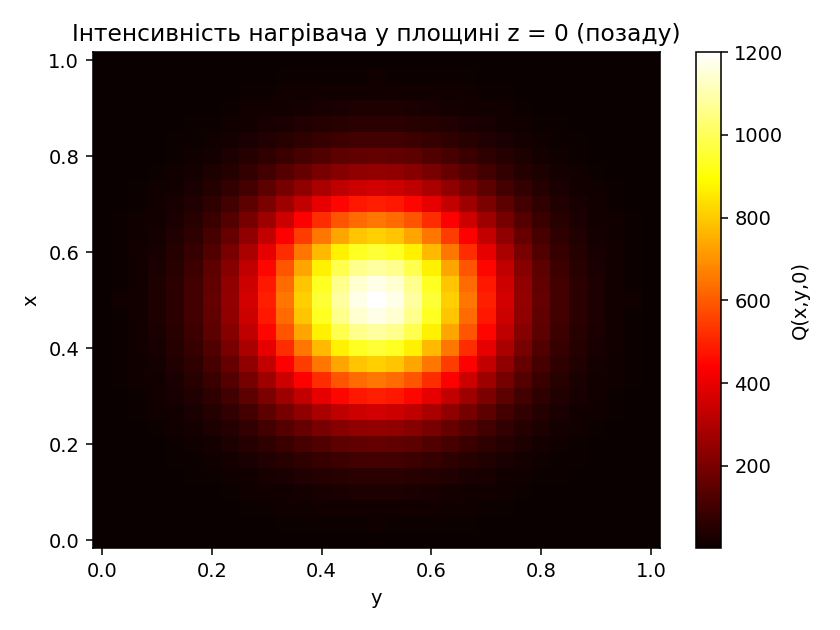
\includegraphics[width=0.6\linewidth]{heater_3d.png}
  \caption{Інтенсивність джерела $f(x,y,0)$ у площині $z=0$ (задня сторона пластини). Локалізований гауссівський нагрівач у центрі; у коді $Q=1200$ (збільшення $Q$ посилює нагрівання).}
  \label{fig:3d-heater}
\end{figure}

\begin{figure}[H]
  \centering
  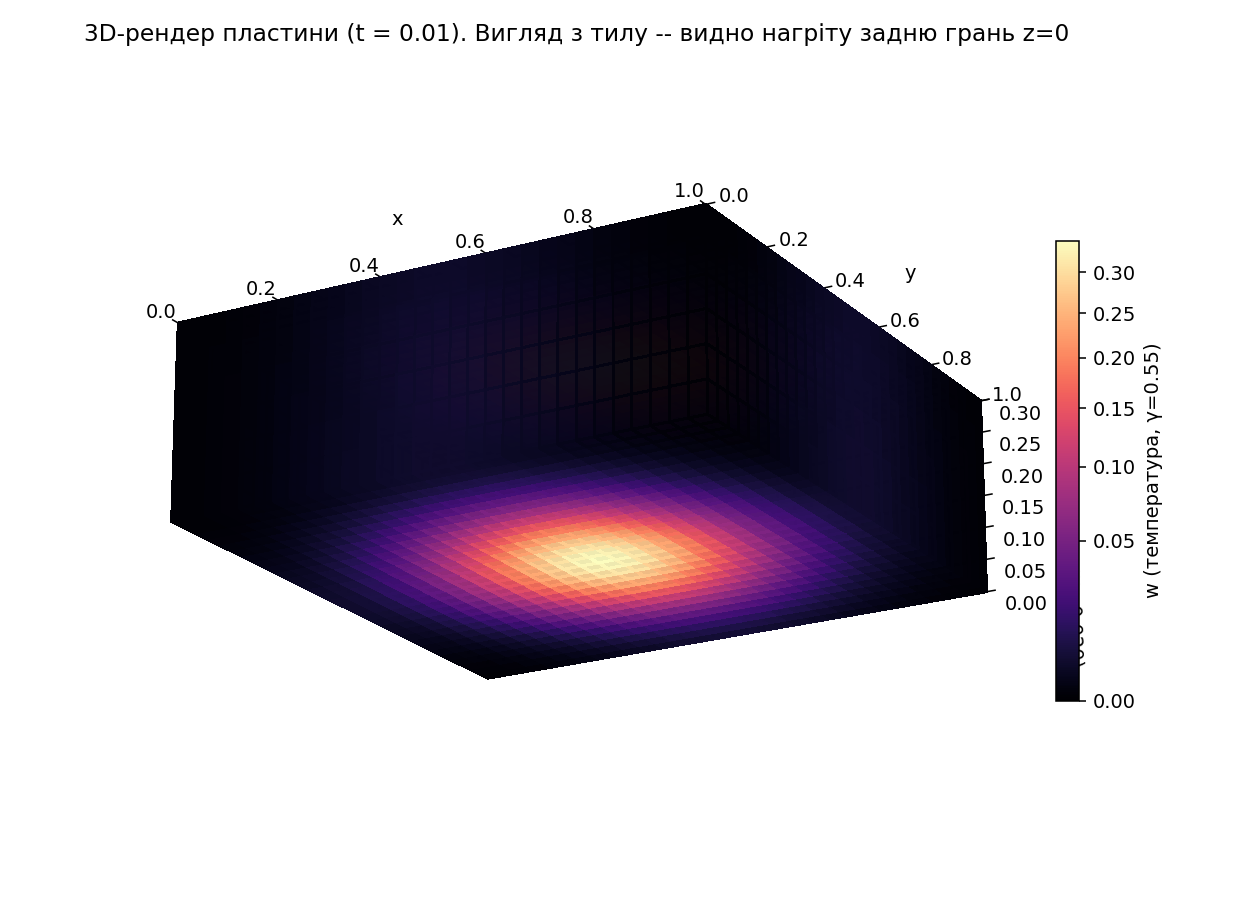
\includegraphics[width=0.85\linewidth]{box_3d.png}
  \caption{3D-рендер пластини-паралелепіпеда $[0,\ell_1]\times[0,\ell_2]\times[0,\ell_3]$ із полем надлишку $w$ на гранях ($t=T$). Задня грань $z=0$ --- нагрівач; передня $z=\ell_3$ --- конвекція \eqref{eq:robin} ($w$ може бути позитивним). Вісь $z$ розтягнуто у $15$ разів для наочності.}
  \label{fig:3d-box}
\end{figure}

\begin{figure}[H]
  \centering
  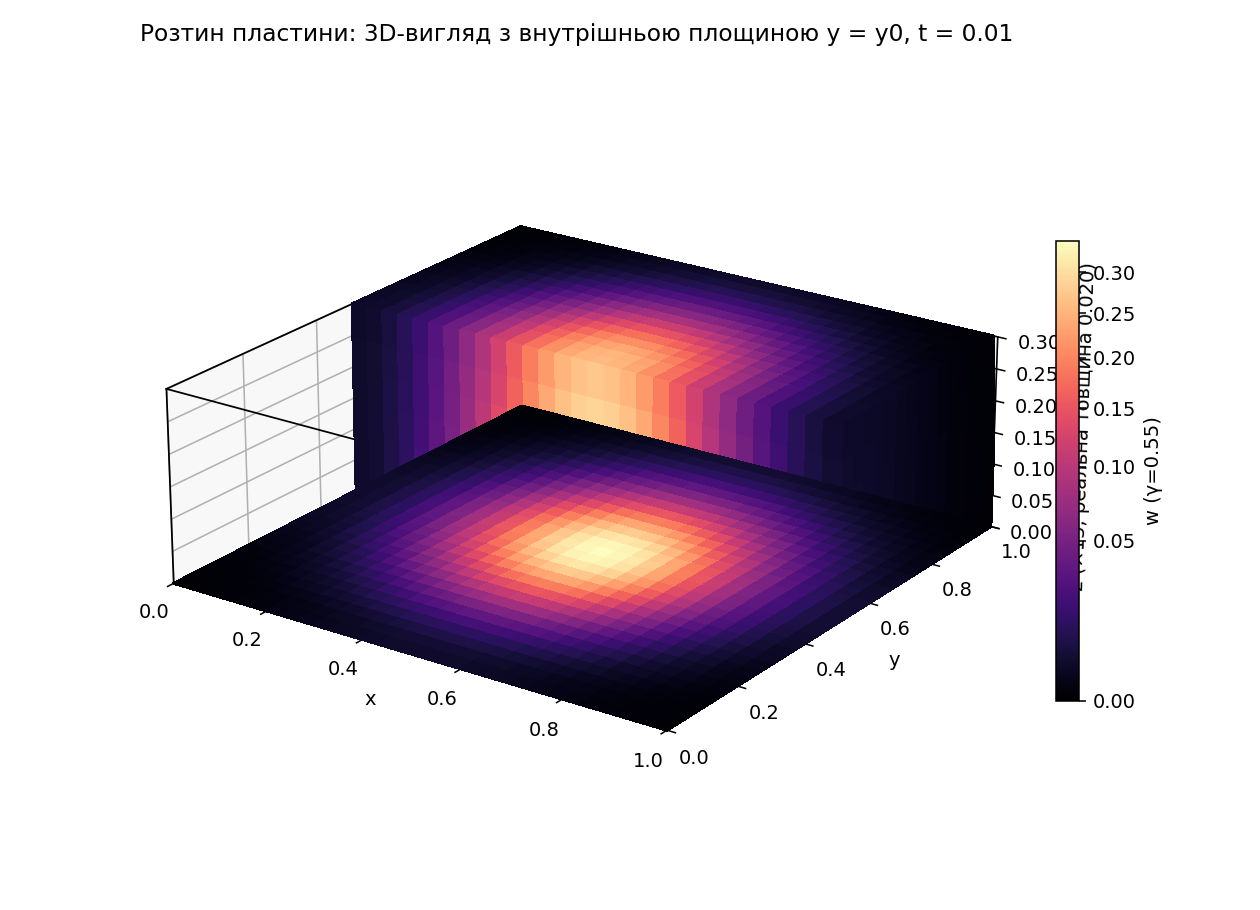
\includegraphics[width=0.85\linewidth]{box_3d_cut.png}
  \caption{Пластина з частковим розтином по площині $y=y_0=1/2$. На задній грані $z=0$ --- максимум нагріву; на передній $z=\ell_3$ --- \emph{ненульовий} надлишок $w>0$ (поверхня тепліша за повітря), бо діє конвекція Ньютона \eqref{eq:robin}, а не ідеальне Дирихле.}
  \label{fig:3d-box-cut}
\end{figure}

\begin{figure}[H]
  \centering
  \noindent\fbox{%
    \begin{minipage}{0.94\linewidth}
      \centering
      \vspace{0.35em}
      {\large\textbf{Інтерактивна 3D-модель (вкладення PDF)}}\\[0.45em]
      \IfFileExists{figures/interactive_3d.html}{%
        \textattachfile[mimetype=text/html,color=0 0 1]{figures/interactive_3d.html}{%
          {\color{blue}\textbf{Відкрити interactive\_3d.html у браузері}}}%
        \\[0.55em]
        {\footnotesize
          Файл \texttt{interactive\_3d.html} (Plotly) \emph{вшито безпосередньо в цей PDF} як вкладення
          (пакет \texttt{attachfile2}). У \textbf{Adobe Acrobat Reader}: клацніть по синьому посиланню вище
          або відкрийте панель вкладень: \texttt{View} $\rightarrow$ \texttt{Show/Hide}
          $\rightarrow$ \texttt{Navigation Panes} $\rightarrow$ \texttt{Attachments}
          (іконка скріпки), оберіть \texttt{interactive\_3d.html}, відкрийте подвійним кліком
          або через контекстне меню. У \textbf{Apple Preview} та багатьох інших переглядачах
          вкладення PDF не підтримуються --- тоді відкрийте той самий файл у каталозі
          \texttt{figures/} або виконайте відповідну комірку в ноутбуці
          \texttt{heat\_equation\_2d.ipynb}.}%
      }{%
        {\footnotesize
          \textbf{Увага.} Файл \texttt{figures/interactive\_3d.html} не знайдено.
          Згенеруйте його перед компіляцією PDF (з каталогу \texttt{lr1}):\\
          \texttt{python3 figures/\_make\_interactive\_3d.py}%
        }%
      }
      \vspace{0.35em}
    \end{minipage}%
  }
  \caption{Інтерактивна 3D-сцена: обертання мишею, масштаб, слайдер часу, кнопки Play/Pause, перемикач розтину.
    Дані збігаються з розділом Д.3 та з ноутбуком \texttt{heat\_equation\_2d.ipynb}.}
  \label{fig:3d-embedded-html}
\end{figure}

\begin{figure}[H]
  \centering
  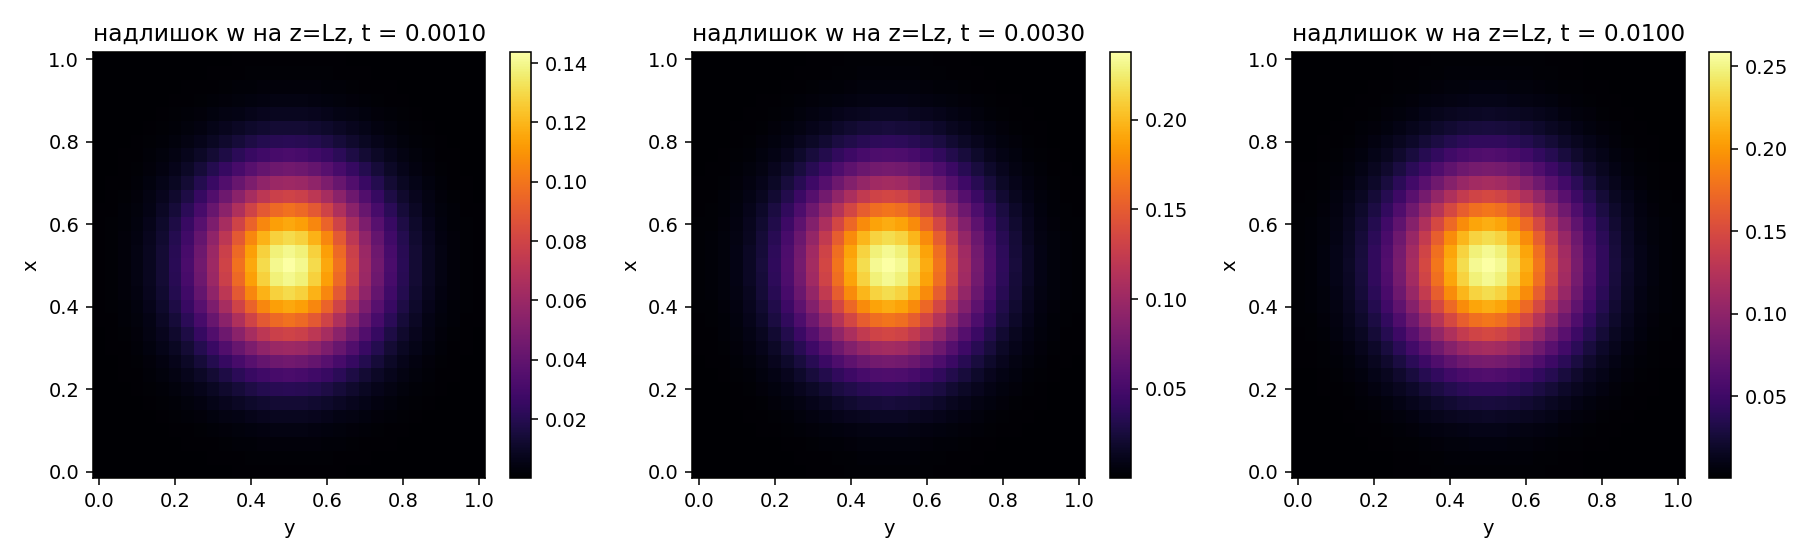
\includegraphics[width=0.98\linewidth]{front_face_3d.png}
  \caption{Надлишок температури $w$ на \emph{передній} поверхні $z=\ell_3$ (без шару ``$-\,h_z$''): конвекція до кімнати; $w>0$ --- пластина тепліша за повітря. Амплітуда менша, ніж біля нагрівача на задній грані, але не нульова.}
  \label{fig:3d-front}
\end{figure}

\begin{figure}[H]
  \centering
  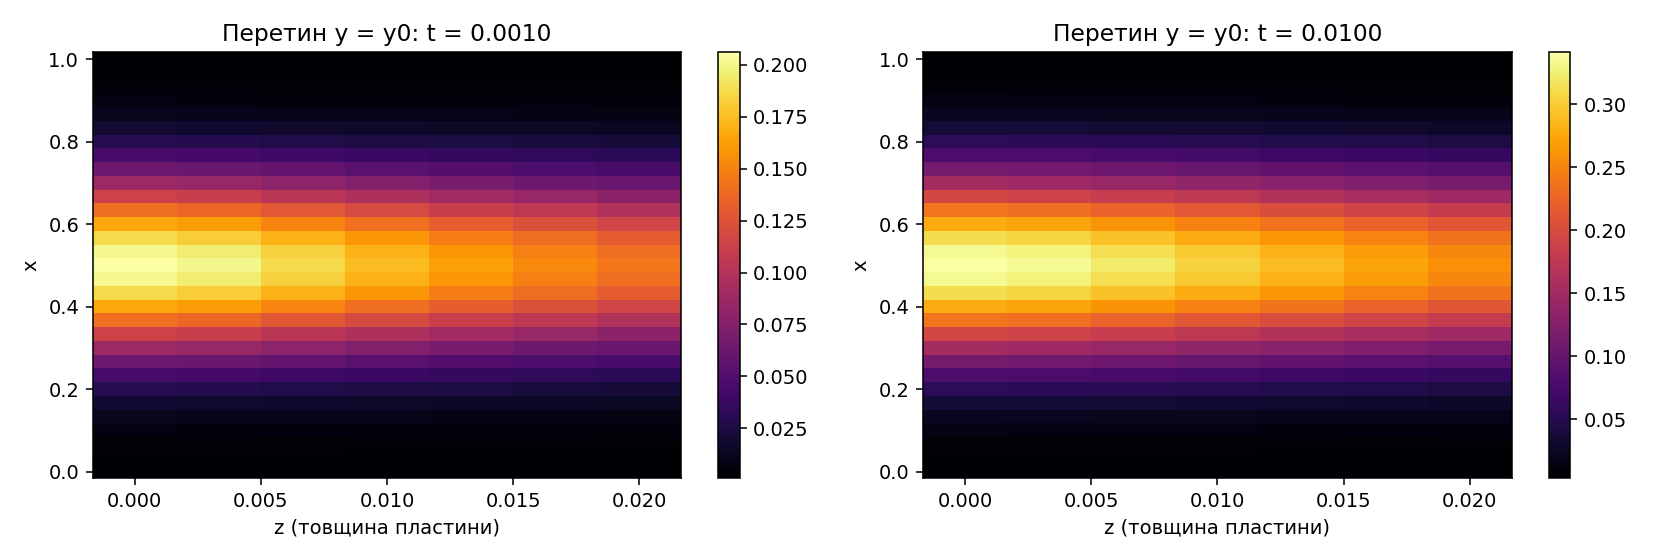
\includegraphics[width=0.98\linewidth]{cross_section_3d.png}
  \caption{Поздовжній перетин у площині $y=y_0$, координати $(x,z)$. Градієнт від нагріву біля $z=0$ до менших значень біля $z=\ell_3$; на передній грані $w>0$ (конвекція до повітря). Масштаб по $z$ у $50$ разів менший за $x$ --- пластина дуже тонка.}
  \label{fig:3d-cross}
\end{figure}

\begin{figure}[H]
  \centering
  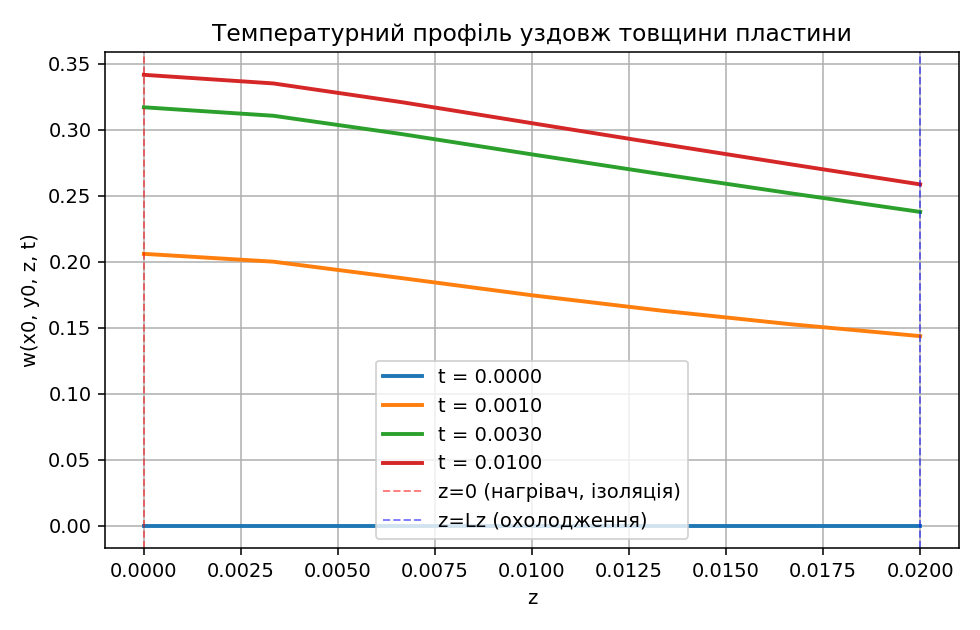
\includegraphics[width=0.75\linewidth]{z_profile_3d.png}
  \caption{Профіль надлишку $w$ уздовж $z$ через центр нагрівача. На передній грані $w(\ell_3)>0$: поверхня тепліша за повітря; умова Робена \eqref{eq:robin} замінює нефізичне $w(\ell_3)=0$.}
  \label{fig:3d-zprof}
\end{figure}

\begin{figure}[H]
  \centering
  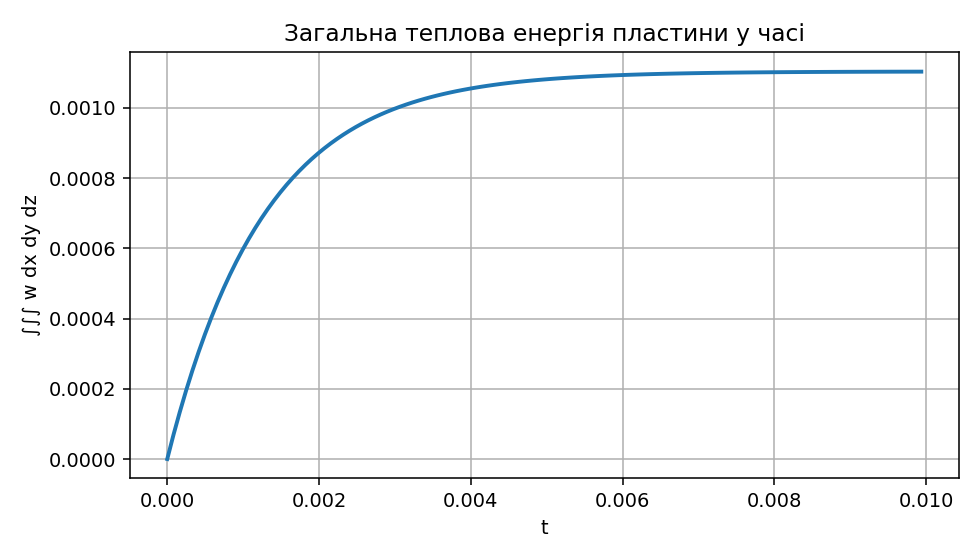
\includegraphics[width=0.75\linewidth]{energy_3d.png}
  \caption{Інтегральний надлишок $\iiint w\,dx\,dy\,dz$ у часі. При конвекції спереду енергія може виходити на плато: приплив від джерела зрівноважується тепловіддачею через передню грань (не миттєвим ``обнуленням'' температури).}
  \label{fig:3d-energy}
\end{figure}

\paragraph{Фізична інтерпретація результатів.}
\begin{itemize}
  \item Повна ізоляція позаду і по бічних гранях унеможливлює тепловтрати через ці поверхні: градієнт $\partial w/\partial n = 0$ чітко видно з плоских профілів біля $z=0$ на рис.~\ref{fig:3d-zprof}.
  \item Тепловий стік -- передня сторона ($z=\ell_3$) через конвекцію \eqref{eq:robin}. У стаціонарі баланс: інтеграл нормального потоку $\propto \iint w\,dx\,dy$ на цій грані узгоджується з повною потужністю джерела в об'ємі.
  \item Через малу товщину пластини ($\ell_3 = 1/50$) характерний дифузійний час у напрямку $z$ складає $\ell_3^2/a \approx 4\cdot 10^{-4}$, тому профіль по товщині встановлюється дуже швидко порівняно з часовим масштабом у площині. Це -- типова ситуація для \emph{тонких пластин}: фактично задача редукується до 2D-задачі для усередненого по $z$ поля, а третій вимір відіграє роль ``перенесення'' тепла від нагрівача до холодильника.
\end{itemize}

\paragraph{Порівняння 2D vs 3D.}
\begin{itemize}
  \item \emph{Стійкість.} Через $h_z \ll \hx$ CFL-крок у 3D обмежений величиною $\sim h_z^2/(2a)\approx 5\cdot 10^{-6}$, тобто у 25 разів жорсткіший за 2D при тих самих $N_x,N_y$. Це -- типова ситуація анізотропних сіток і головна причина використовувати неявні схеми (ADI, LOD) для тонких пластин.
  \item \emph{Обчислювальна вартість.} Зростає як $N_x N_y N_z$ (на крок) разом із зростанням кількості кроків за CFL. У нашій реалізації $4590$ кроків замість $40$ в ADI-2D, тобто різниця на два порядки.
  \item \emph{Фізика.} Третій вимір дає змогу врахувати розділення ``гарячої'' (задньої) і ``холодної'' (передньої) сторін пластини -- чого 2D-усереднена модель не відтворює. Саме це відповідає реальній постановці тепловідводу від мікросхеми, нагрівача тощо.
  \item \emph{Ефективні алгоритми.} ADI та DS-LOD природно узагальнюються на 3D (Douglas--Gunn ADI, триетапне розщеплення); неявні схеми особливо вигідні для анізотропних сіток, бо зберігають безумовну стійкість незалежно від співвідношення $\hx / h_z$.
\end{itemize}

% ===================================================================
\section*{Висновки (загальні)}
\addcontentsline{toc}{section}{Висновки (загальні)}
% ===================================================================

\begin{enumerate}
  \item Побудовано та програмно реалізовано три різницеві схеми (явну, ADI, двокрокову симетризовану DS-LOD) для 2D рівняння теплопровідності у стилі позначень статті [Грищенко, Оноцький, 2000]; отримано погодженість $O(\hx^2+\tauh^{p})$, $p\ge 1$, та стабільність при дотриманні CFL-умов.
  \item На тестовому гауссівському розв'язку (варіант 5) усі три методи дають похибку не більше $3\cdot 10^{-5}$, що підтверджує коректність реалізації.
  \item ADI -- оптимальний за швидкодією метод для розглянутої задачі; явна схема -- проста, але з жорстким обмеженням на $\tauh$; DS-LOD має перспективи для складніших рівнянь.
  \item Експерименти з граничними умовами ілюструють фізичні відмінності: охолодження (тепловідвід) проти ізоляції (збереження енергії).
  \item Розширення до 3D підтверджує загальні закономірності параболічних задач і наочно демонструє, чому в $3D$ особливо цінні неявні схеми.
\end{enumerate}

% ===================================================================
\section*{Список літератури}
\addcontentsline{toc}{section}{Список літератури}
% ===================================================================

\begin{enumerate}
  \item Грищенко О.Ю., Оноцький В.В. \emph{Дисипативність двокрокових симетризованих алгоритмів для гіперболічних рівнянь переносу} // Вісник Київського університету. Сер.: фіз.-мат. науки. -- 2000. -- Вип. 3. (див. ARTICL60.pdf).
  \item Peaceman D.W., Rachford H.H. \emph{The numerical solution of parabolic and elliptic differential equations} // J. SIAM. -- 1955. -- Vol. 3(1). -- P. 28--41.
  \item Strang G. \emph{On the construction and comparison of difference schemes} // SIAM J. Numer. Anal. -- 1968. -- Vol. 5(3). -- P. 506--517.
\end{enumerate}

\end{document}
